% !TeX root = RJwrapper.tex
\title{Capitalized Title Here}
\author{by Author One, Author Two}

\maketitle

\abstract{%
An abstract of less than 150 words.
}

\hypertarget{real-rata-and-simulations}{%
\subsection{Real Rata and Simulations}\label{real-rata-and-simulations}}

\hypertarget{boston-housing-data}{%
\subsubsection{Boston Housing data}\label{boston-housing-data}}

\begin{Schunk}
\begin{Sinput}
#source the functions. Will be changed to load package
source("../R/SINDEXQ_fun.R")

#load data from MASS
library(MASS)
#help(Boston)
medv<- Boston$medv
RM <- Boston$rm
logTAX <- log(Boston$tax)
PTRATIO <- Boston$ptratio
logLSTAT <- log(Boston$lstat)

X <- cbind(RM,logTAX,PTRATIO,logLSTAT)
y0<-medv - mean(medv)

#result is not the same with Wu 2010 as initial was not normalized in Wu 2010
#tianhai
#beta0 <- c(1,-1,0,-1);
beta0 <- NULL
tau.vec <- c(0.2,0.5,0.8)
est.coefficient <- matrix(NA, nrow = length(tau.vec), ncol = 5)
est.coefficient[,1] <- tau.vec
for (i in 1:length(tau.vec)){
  est <- siqr(y0,X,beta.inital = beta0, tau=tau.vec[i],maxiter = 20,tol = 1e-6)
  est.coefficient[i,2:5] <- est$beta
}
colnames(est.coefficient) <- c("quantile tau",colnames(X))
est.coefficient
\end{Sinput}
\end{Schunk}

\begin{Schunk}
\begin{Sinput}
est.tau02 <- siqr(y0,X,beta.inital = NULL, tau=0.2)
plot.si(est.tau02,bootstrap.interval = TRUE)
\end{Sinput}
\end{Schunk}

\begin{Schunk}
\begin{Sinput}
est.tau05 <- siqr(y0,X,beta.inital = NULL, tau=0.5)
plot.si(est.tau05,bootstrap.interval = TRUE)
\end{Sinput}
\end{Schunk}

\begin{Schunk}
\begin{Sinput}
est.tau08 <- siqr(y0,X,beta.inital = NULL, tau=0.8)
plot.si(est.tau08,bootstrap.interval = TRUE)
\end{Sinput}
\end{Schunk}

\hypertarget{simulation}{%
\subsubsection{Simulation}\label{simulation}}

\begin{Schunk}
\begin{Sinput}
n <- 400
beta0 <- c(1, 2)/sqrt(5)
n.sim <- 100
tau <- 0.5

data <- generate.data(n, true.theta=beta0, setting = "setting3",ncopy = n.sim)

#paralell 
library(parallel)
library(foreach)
cl<- makeCluster(12)
doParallel::registerDoParallel(cl)
sim.results <- foreach(m = 1:n.sim,.combine = "rbind") %dopar% {
  X <- data$X
  Y <- data$Y[[m]]
  est <- siqr(Y, X, beta.inital = NULL, tau=tau,maxiter = 30,tol = 1e-8)
  est$beta
}
\end{Sinput}
\end{Schunk}

\begin{Schunk}
\begin{Sinput}
tau <- 0.5
sim.results <- readRDS("./sim.results.RDS")
est.mean <- c(tau,apply(sim.results,2,mean))
names(est.mean) <- c("tau","beta1.hat","beta2.hat")
est.mean
\end{Sinput}
\begin{Soutput}
#>       tau beta1.hat beta2.hat 
#> 0.5000000 0.4515909 0.8917233
\end{Soutput}
\end{Schunk}

\begin{Schunk}
\begin{Sinput}
est.se <- c(tau,apply(sim.results,2,sd))
names(est.se) <- c("tau","beta1.se.hat","beta1.se.hat")
est.se
\end{Sinput}
\begin{Soutput}
#>          tau beta1.se.hat beta1.se.hat 
#>   0.50000000   0.02682211   0.01359602
\end{Soutput}
\end{Schunk}

\begin{Schunk}
\begin{Sinput}
boxplot(data.frame((sim.results)), outline=T,notch=T,range=1,main = "Boxplots of Coefficient Estimates (100 replications)",horizontal = F)
\end{Sinput}

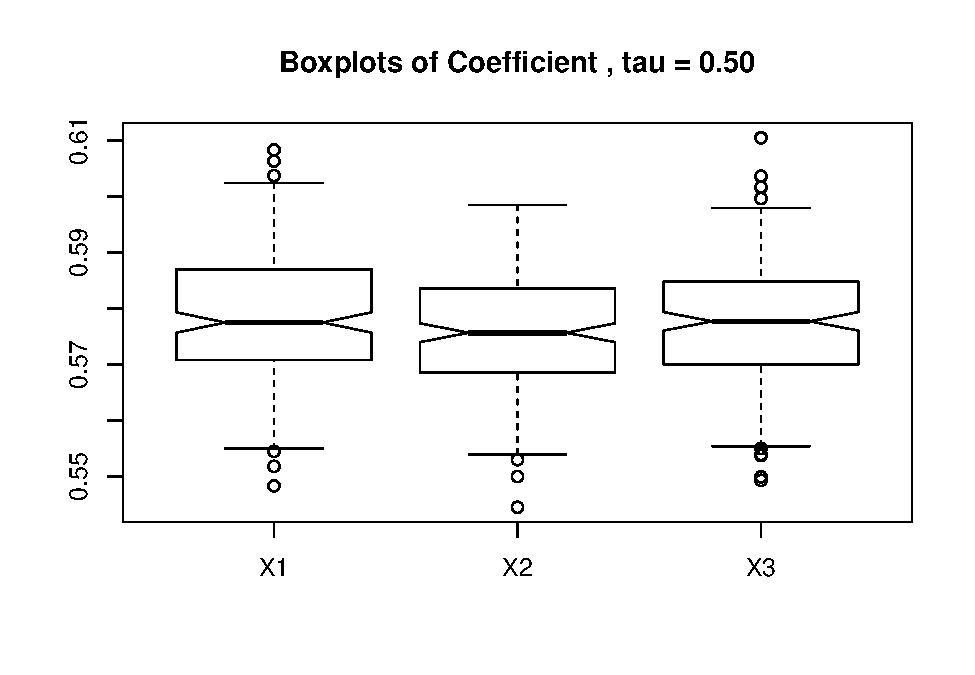
\includegraphics{siqr_files/figure-latex/unnamed-chunk-8-1} \end{Schunk}

\begin{Schunk}
\begin{Sinput}
est.sim.05 <- siqr(data$Y[[1]],data$X,beta.inital = NULL, tau=0.5)
plot.si(est.sim.05,bootstrap.interval = TRUE)
\end{Sinput}
\end{Schunk}

\begin{Schunk}
\begin{Sinput}
Sys.sleep(100)
\end{Sinput}
\end{Schunk}

\bibliography{RJreferences}


\address{%
Author One\\
Affiliation\\
line 1\\ line 2\\
}
\href{mailto:author1@work}{\nolinkurl{author1@work}}

\address{%
Author Two\\
Affiliation\\
line 1\\ line 2\\
}
\href{mailto:author2@work}{\nolinkurl{author2@work}}

